
\chapter{ State of art \\
Internet Industriel des Objets (IIoT)}
\section{Introduction}
The IoT has disrupted numerous industries by making devices secure, intelligent and connected; it enables process optimization and provides data-driven decision making. For my first foray into the Internet of Things, I learned fundamental skills for designing and integrating connected systems. From this experience I was then able to progress onto a higher level, that of the IIoT (Industrial Internet of Things) where I could take my initial learnings, and focus them towards more complex industrial application-focussed environments.
\begin{figure}[H]
    \centering
    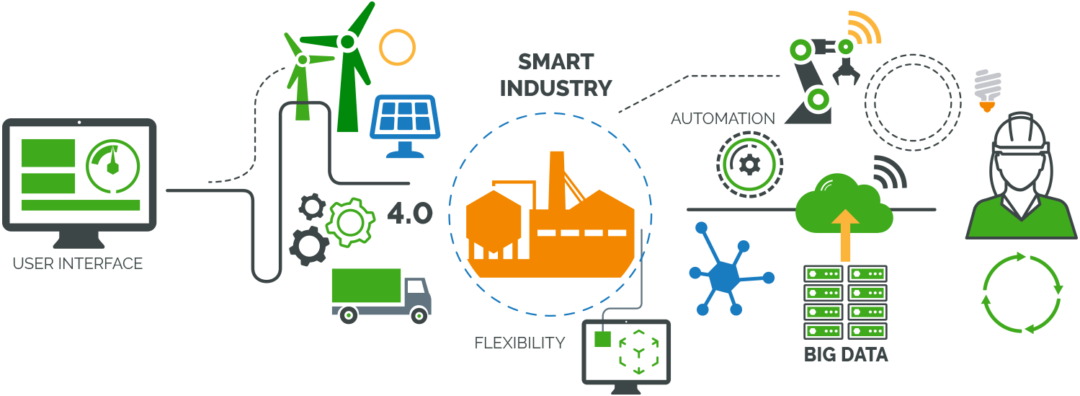
\includegraphics[width=0.7\textwidth]{chapters/N-1/img/what-is-industrial-Internet-of-things-1080x396.png}
    \caption{Somfy Zriba Products}
    \label{fig:campus}
\end{figure}

\section{L’IoT et l’IIoT}
While the principles behind IoT and IIoT are similar, their requirements are different. IoT is mostly aimed at consumers, whereas IIoT is for industrial setups such as manufacturing, energy and infrastructure. In my case, this transition from IoT to IIoT was important because now I am trying to solve some technical challenges like system resilient, more secure and real-time data handling.

\section{Les architectures de référence}
Robust reference architectures are the foundation upon which IIoT operates, and they are created to ensure seamless interoperability, securing system scale. These models can be one of the three-tier architecture (perception, network and application) model which provide a systematic way to govern data stream from sensors up-to analysis and visualization platform. These principles are utilized in this project, where secure gateways relay data from industrial sensors to advanced processing systems.

\section{Qualité de service dans l'IIoT}
Quality of Service (QoS) is an essential aspect in IIoT systems that ensures performance, dependability and confidentiality communications. In an industrial environment, a minor failure or delay results in significant losses. As part of my IIoT exposure I had to pay close attention to various QoS mechanisms, specially for realtime monitoring of industrial equipment that needs immediate and timely transfer of data.